\chapter{Tools and their artefacts}~\label{chapter-tools-and-their-artefacts}
%\julian{This chapter covers \utools and \itools.}

This chapter covers two of the six perspectives, \emph{i.e.} using and improving mobile analytics tools. The primary evidence comes from both the app-centric and the tools-centric case studies, augmented with material from grey data and grey literature.

The evidence has been analysed and prioritised to keep the chapter relatively succinct and on topic. 38 L1 themes emerged in the analysis of the evidence, of these the ones with strongest support in terms of the evidence are included here, the rest would benefit from further work.

The top ranked L1 themes are core to this chapter and they are: 
{\small
\begin{enumerate}
    \itemsep0em
    \item[1] sdk-design: the design of the client-side SDK affects many aspects of the data collection which then feeds subsequent stages in the processing of the data to provide the mobile analytics.
    \item[1] ux-design: The design of the User Experience (UX) of the mobile analytics tool for their audience of the software development team (and particularly the app developers).
    \item[3] product-fit: whether, and if practical how well, the mobile analytics product fits the desires/needs of the developers. 
    \item[4] actionable-reports: reports the developers can action in order to address concerns presented in the reports.    
    \item[4] integration-into-workflows: the ability of a given mobile analytics tool/service to be integrated into development team's workflows.
    \item[6] meta-data: data not directly about the app, instead it's data about the user and/or their device, etc.
    \item[7] flaws: weaknesses, mistakes, errors, etc. pertaining to the mobile analytics tool/service.
    \item[8] ethical-considerations: the data collected by mobile analytics may have ethical implications a) for the operator/provider of the service, b) for their partners and customers, c) for the developers, d) for end-users. In this research our main focus is on the implications for the developers, nonetheless the other aspects are also important.
    \item[8] link-rot-preservation-of-results: the validity of a URL may be finite, as may the contents be even if the link remains. For mobile analytics services link rot is often a common reason why results are no longer available from the mobile analytics service - the link was ephermeral. In such cases the results would need to be preserved while the results are still available. In some cases the rot may be easy to predict, for instance as data ages beyond the predefined date range of a report, in other cases less so, for instance when the active release is updated the data for the previous currently active release might 'disappear' from some reports.
    \item[10] benefits-of-combining-mobile-analytics-tools: an observation of benefits developers can obtain through combining their use of several mobile analytics tools.
    \item[11] bug-localisation: features in the tool that may enable developers to localise one or more bugs.
    \item[12] efficacy-of-tool: how efficient and how effective is the tool, i.e. how efficacious is the tool? Did it achieve the objectives it claims to achieve?
    \item[12] engineering-challenges: Engineering challenges related to developing the components of the mobile analytics tool/service such as provision of a client-side SDK that collects failures for native (C++) code.
    \item[12] return-on-investment: developers may make both implicit and explicit choices on what to invest in, for instance in terms of their focus, their effort, and their money. The analytics tools need to convince developers a) to invest and then b) whether to increase that investment (and if so what forms of investment e.g. in terms of writing more code, spending [more] money, using the tool more, etc.).
    \item[12] testability: the ability to test the overall service, the tool, and/or components that comprise the analytics tool.
    \item[12] vying-for-attention-of-developers: mobile analytics competes (vies) for the attention of the app developers against a plethora of other competing demands, offerings, and constraints. 
\end{enumerate}
}

These can be aggregated into four higher-level (L2) themes: design (\secref{section-design}), fit-for-purpose (\secref{section-fit-for-purpose}), utility (\secref{section-utility}), dependability (\secref{section-dependability}). Figure \ref{fig:analytics-tools-and-their-artefacts-fishbone-diagram} illustrates the top L1 themes and their main higher-level (L2) theme.
\begin{figure}
    \centering
    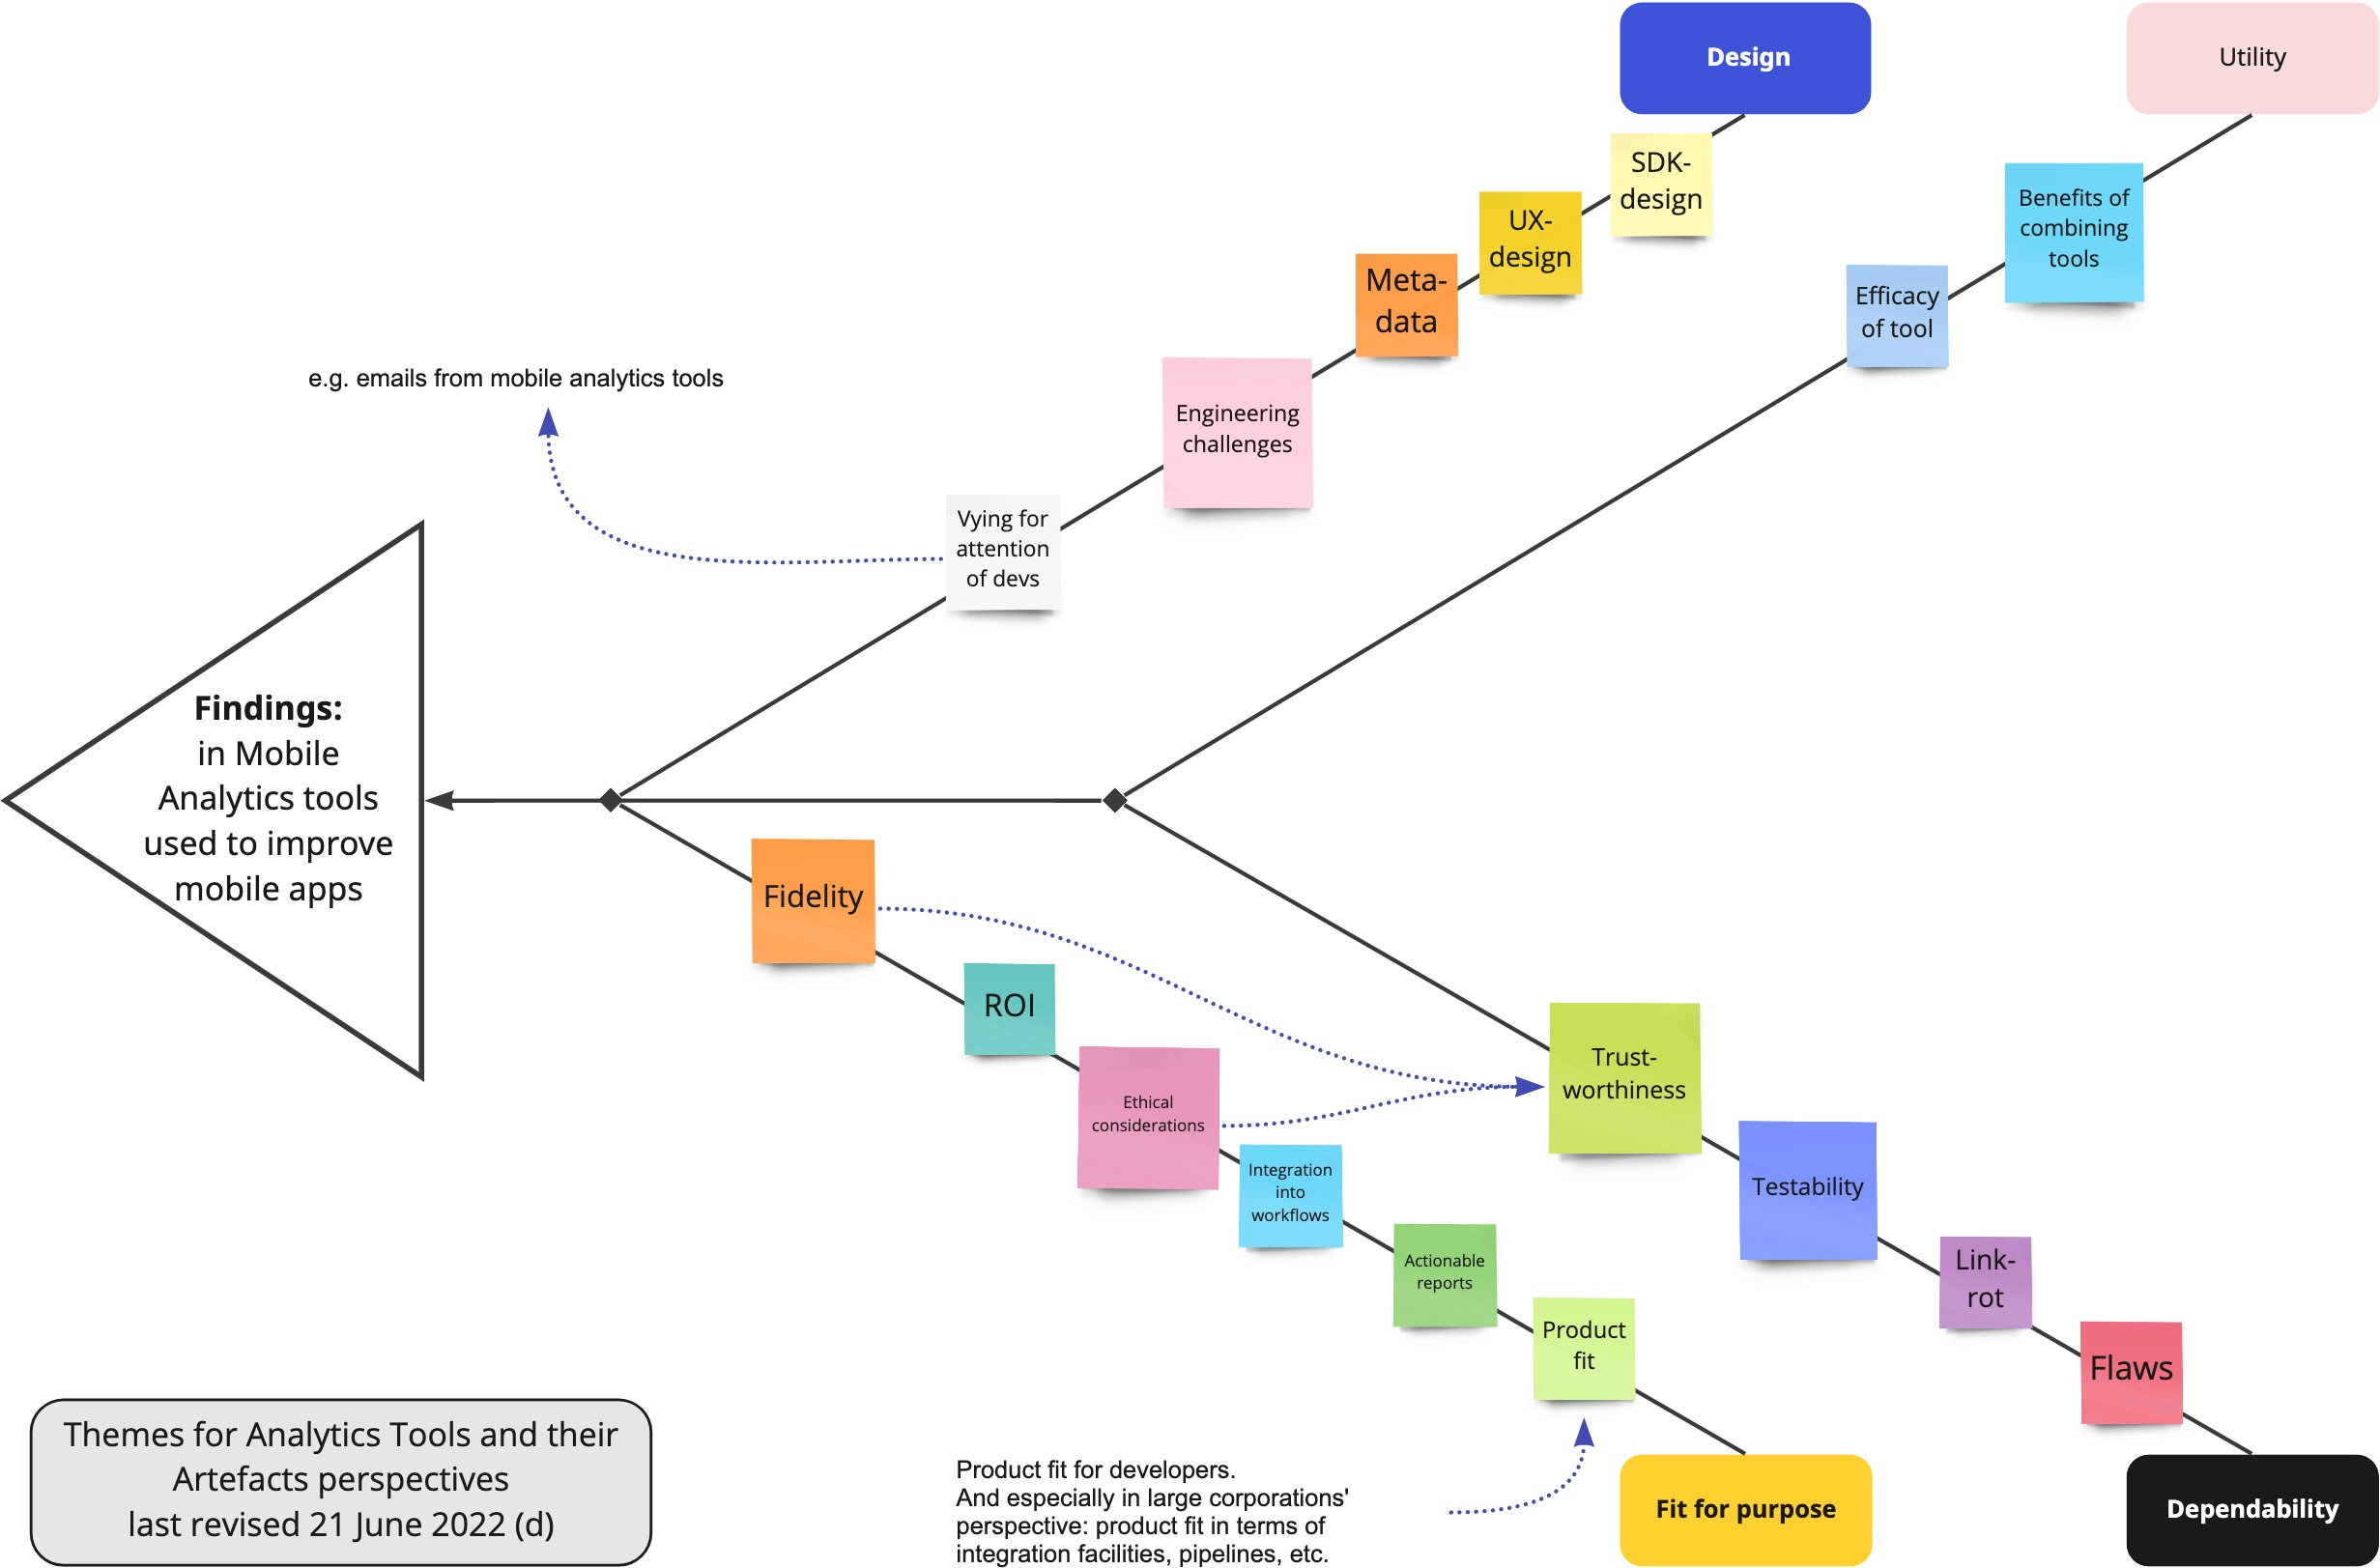
\includegraphics[width=\textwidth]{images/rough-sketches/analytics-tools-and-their-artefacts-fishbone-diagram-21-jun-2022d.jpeg}
    \caption{Analytics Tools and their Artefacts Fishbone Diagram\\Source: \href{https://miro.com/app/board/uXjVOtIsyWo=/?share_link_id=293061080490}{Miro}}
    \label{fig:analytics-tools-and-their-artefacts-fishbone-diagram}
\end{figure}

\section{Design}~\label{section-design}
Design of the SDK, see \ref{section-sdk-design}, and the developer-experience (UX), see \ref{section-developer-experience-ux-design}, of the mobile analytics emerged as the top two ranked themes for analytics tools. Any in-app SDK needs to integrate easily in to the mobile app and platform-level analytics needs to be seamless and collect sufficient pertinent information to be useful for the app developers. They also need to be robust and timely in terms of collection, transmission, and processing of the underlying data in order for developers to have timely access to the results. 

Fabric Crashlytics is an archetypal example of how a mobile analytics tool can be designed to serve developers well. The product team developed it from the ground up, starting with excellent crash reporting, to provide developers with timely, actionable, attractive, and useful reports. This led to it becoming one of the top three mobile analytics tools for both iOS and Android within 10 months of being launched~\citep{___answersblog_2015_may_crashlytics-no1-in-performance}. % See also https://web.archive.org/web/20151203150947/http://fabric.io/blog/crashlytics-answers-named-top-mobile-sdks
First Twitter acquired it and then Google did; they subsequently integrated it into Firebase Analytics which is the most popular mobile analytics service for Android apps currently.

Platform-level analytics provides an outsider's perspective on the behaviour of mobile app, in contrast to in-app analytics that provides an insider's perspective. In this research Google's Android Vitals provides the platform-level analytics as it has the largest reach of any platform-level analytics across the widest range of devices. The platform provides users the ability to allow or deny analytics to be sent from their device. Apple's iOS (and MacOS) ask the user explicitly~\citep{apple_ios_share_diagnostics}, Android does not - users need to find the setting and opt-out~\citep{google_play_share_usage_and_diagnostics_info_with_google}. % See also https://chefkochblog.wordpress.com/2018/02/09/how-to-disable-android-usage-diagnostics-sharing/ I've not referenced this as they don't provide evidence of the default settings.

Mobile Analytics tools vie for attention against a plethora of other developer-oriented tools, project demands, \emph{etc.} Developers need to be enticed into using the tools and then retained on an ongoing basis to meet the objectives of the providers of the mobile analytics services.

\subsection{SDK design}~\label{section-sdk-design}
Any mobile analytics SDK needs to be designed to collected relevant data and forward that data so it can be processed, analysed, and reported on. 

\textbf{Programming language support}: 
Mobile apps %are written using hybrid/cross platform-frameworks, others in platform/managed code, a few may be written purely in native/unmanaged code, and some combine several of these. They 
can be written in several programming languages. While many mobile apps are written in a single programming language some use several programming languages, for instance Kiwix Android combines Java, Kotlin, and C++. 
% More reading on Cordova's demise: https://medium.com/codex/the-sunset-of-apache-cordova-alternatives-for-cross-platform-mobile-development-in-2022-9da34234c992

Mobile analytics SDKs, in turn, support one or more of the programming languages. If they do not support the programming languages then they may not be able to obtain or provide analytics for elements written in the unsupported programming languages. For C and C++ code in particular, the app developers generally need to explicitly configure the code and the build process to incorporate the relevant mobile analytics SDK if it's available. % For a counterexample Fabric Crashlytics claimed their SDK was very easy to integrate https://web.archive.org/web/20151019132428/https://crashlytics.com/blog/the-wait-is-over-launching-crashlytics-for-android-ndk

\textbf{SDK initialisation}: 
The SDK needs to be initialised as early as practical each time the app is started (or restarted) if it's to capture pertinent information (including crashes that occur when the app starts or restarts). For mobile analytics SDKs this has led to their developers finding and implementing mechanisms to initialise their SDK in innovative (and unusual) ways, for instance Firebase uses a ContentProvider~\citep{stevenson2016_how_does_firebase_initialize_on_android}. Note: this does not always work, as reported in \citep{reddy2022_crashlytics_fails_to_track_app_startup_crashes}. When the SDK initialises it obtains various meta data about the app and the device. 

\textbf{Data automatically collected by SDKs}
The mobile analytics SDKs have collected data automatically for years, the developers do not need to write additional code to collect this data. The data includes meta-data, for instance about the device and version of the platform. Depending on the SDK it may also collect demographic data, sensor data such as the geo-location, other data such as other apps that are installed, and various events that occur including network requests and responses. The data collected is covered shortly in \ref{section-meta-data}.

Any of these data elements \textit{may} help developers to improve their software, however, use of this data may be considered a privacy risk, particularly for end-users and may lead to ethical conundra for the development team and their organisation.\pending{Link to the ethics material.}

\textbf{Runtime activities for the SDK}: 
When the SDK is running, which they do in the background without being visible to the user of the app, they are responsible for the safekeeping and transmission of the collected data. Some collect data automatically, or autonomously. For example, Sentry's in-app SDK collects `automatic instrumentation'~\citep{sentry2021_mobile_vitals_four_metrics_every_mobile_developer_should_care_about}, and Android Vitals collects usage data, app crashes, and ANRs automatically.

At least some of the SDKs store analytics data locally on the device on an interim basis, the stored data would be removed once it had been successfully transmitted. Various SDKs limit the number of items they store. The SDKs also vary in how and when they transmit the data and on their behaviour if there isn't a suitable network connection to transmit the data.

\textbf{Limitations in visibility by an SDK}: 
In short, the viewpoint of the SDK affects and can limit what it can observe/record. Also some mobile apps incorporate their own runtime which may hide some failures from being observed by the platform.

\textbf{Android Vitals}: 
Android Vitals does not collect crashes that are contained within an application's runtime. React-Native is a popular cross-platform app development framework. It includes its own application runtime environment and this runtime automatically restarts the app if it crashes. These crashes are not visible to Android Vitals as evidenced by two of the apps within the app centric case studies: LocalHalo and Taskinator where Android Vitals showed no crashes for either these apps, with one exception. 

\textbf{Some failures did emerge}:
That exception was when Android Vitals did report crashes in March and April 2020. Figure \ref{fig:localhalo-android-vitals-no-data-16-march-2020} was recorded on \nth{16} March 2020 before these started and shows the App Health Overview page with a link to a video introducing Android Vitals~\footnote{This appears as a mainly black rectangle in this thumbnail screenshot.}, and the App Health Details page with no data.

\textbf{In-app analytics support for detecting ANRs}: 
Conversely, in-app analytics SDKs were not able to measure ANRs which meant Android Vitals was the primary source of ANR analytics for Android app developers~\footnote{There is an opensource utility that uses a watchdog timer to detect ANRs~\citep{salomonbrys_github_anr_watchdog}. Investigating it was beyond the scope of the immediate research, nonetheless Sentry used that code as a basis for their ANR reporting (\href{https://github.com/getsentry/sentry-java/blob/3f8d7b1cc869bb056c9db99b459e43f6c375784a/sentry-android-core/src/main/java/io/sentry/android/core/ANRWatchDog.java}{sentry-android-core...ANRWatchDog.java}).}. 

Note: Google has subsequently added a mechanism to enable apps to obtain information about previous ANRs when the app next started. The method is \href{https://developer.android.com/reference/kotlin/android/app/ActivityManager#gethistoricalprocessexitreasons}{\texttt{getHistoricalProcessExitReasons()}}~\footnote{The source code is available online: \url{https://android.googlesource.com/platform/frameworks/base/+/master/core/java/android/app/ApplicationExitInfo.java} and provides more details of the design and the data structures.}, added in \href{https://developer.android.com/about/versions/11}{Android 11}, API level 30.
% Various discussions and explanations of using this API follow:
% https://commonsware.com/R/pages/chap-dataaccess-002.html - possibly the best and clearest code examples with explanations.
% Announcing the new functionality in 2021 https://firebase.blog/posts/2021/11/whats-new-at-Firebase-Summit-2021
% https://medium.com/@yangweigbh/monitoring-app-termination-on-android-11-97d514a3f9 
% Facebook's SDK to obtain cached ANRs https://developers.facebook.com/docs/reference/androidsdk/current/facebook/com/facebook/internal/instrument/anrreport/anrhandler.html/ and https://github.com/facebook/facebook-android-sdk/blob/5fe6e2a9d7056a17f54c1cae13e00788723d34f6/facebook-core/src/main/java/com/facebook/internal/instrument/anrreport/ANRHandler.kt
%
At the time of writing, Firebase Analytics uses this mechanism to obtain the ANR and other app exit data, see \href{https://github.com/firebase/firebase-android-sdk/blob/73131b69b0134456441e7fa218964b6a766fcec7/firebase-crashlytics/src/main/java/com/google/firebase/crashlytics/FirebaseCrashlytics.java}{\texttt{github.com.........FirebaseCrashlytics.java}}.

\subsection{LocalHalo React Native example}
The LocalHalo app-centric case study provides an illustration where app crashes were not observed by Android Vitals until a failure in the React Native runtime occurred.

\begin{figure}[htbp!]
\centering
\begin{minipage}{.45\textwidth}
  \centering
  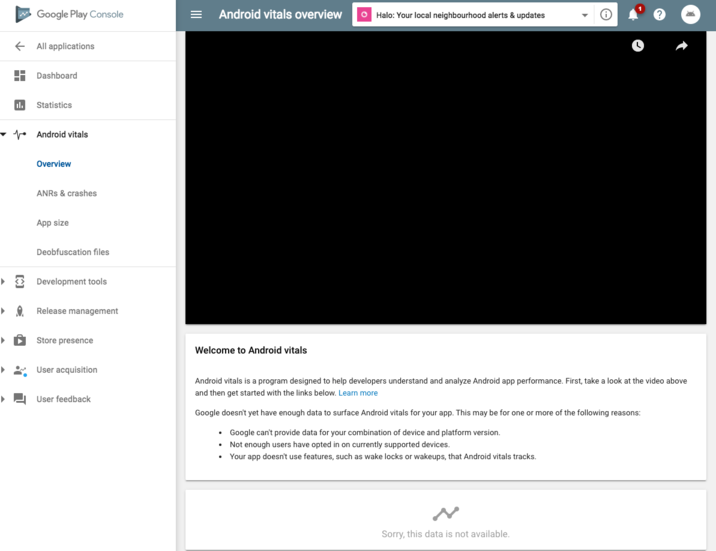
\includegraphics[width=\textwidth]{images/localhalo/apphealthoverviewplace_5550596_no_data.png}
  \captionof*{figure}{App Health Overview page}
\end{minipage}\hfill%
\begin{minipage}{.45\textwidth}
  \centering
  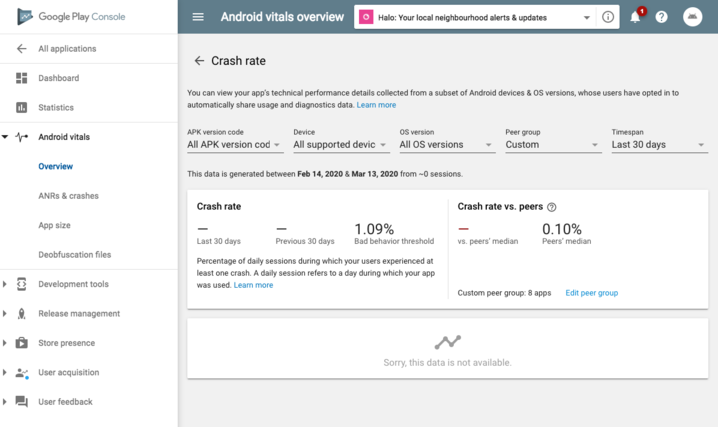
\includegraphics[width=\textwidth]{images/localhalo/apphealthdetailsplace_55505963_no_data.png}
  \captionof*{figure}{App Health Details page}
\end{minipage}
    \caption{No Android Vitals reports on \nth{16} March 2020}
    \label{fig:localhalo-android-vitals-no-data-16-march-2020}
\end{figure}

Figure~\ref{fig:localhalo-android-vitals-high-failures-26-march-2020} was recorded ten days later in \nth{26} March 2020 and shows the alerts for both high crash and ANR rates in the App Health Overview page and the graph for the rampant crash rate in the corresponding App Health Details page. These indicate the failures were related to the native runtime rather than within the React Native code. These were not reported by any Sentry Alerts and they do not appear in the weekly summary reports, except potentially by the absence of data shown in Figure~\ref{fig:sentry-missing-data-march-2020}. While the reason for this was not explained in the interviews or in the analytics data, it is likely that this caused by severe crashes that prevented Sentry's SDK from reporting any data.

\begin{figure}[htbp!]
\centering
\begin{minipage}{.45\textwidth}
  \centering
  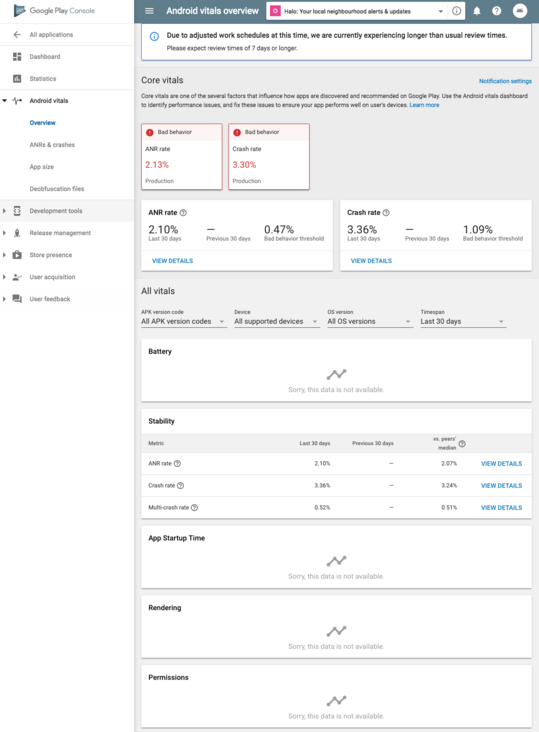
\includegraphics[width=\textwidth]{images/localhalo/apphealthoverviewplace_5550596_high_errors.png}
  \captionof*{figure}{App Health Overview page}
\end{minipage}\hfill%
\begin{minipage}{.45\textwidth}
  \centering
  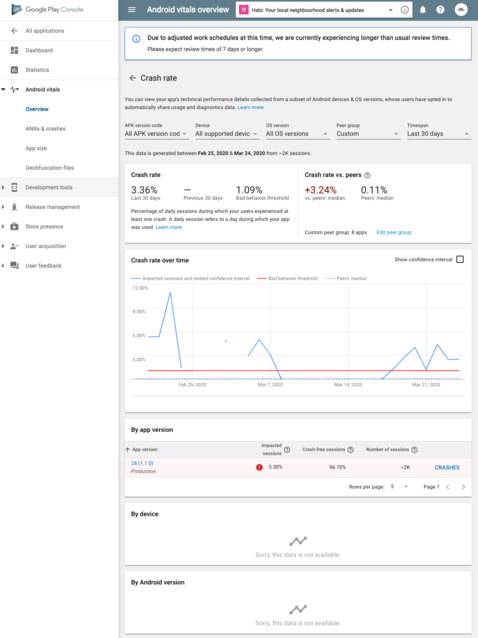
\includegraphics[width=\textwidth]{images/localhalo/apphealthdetailsplace_55505963_high_errors.png}
  \captionof*{figure}{App Health Details page}
\end{minipage}
    \caption{Alerts and graphs in Android Vitals on \nth{26} March 2020}
    \label{fig:localhalo-android-vitals-high-failures-26-march-2020}
\end{figure}

A release in March 2020 had a high crash rate for the production release of their Android app. The top crash cluster was for:

{\small \texttt{java.lang.RuntimeExceptionhost.exp.exponent.experience.a\$b.run}} 

This was traced to a problem in the expo library the development team used in the app~\citep{expo2019_issue5839}~\footnote{Expo is a very popular opensource platform for making universal native apps that run on Android, iOS, and the web \url{https://github.com/expo/expo}.}. In that issue several developers for different Android apps provide data from Google Play Console confirming they also receive similar crash clusters. The cause has not yet been definitively traced or addressed, however for the LocalHalo app the crashes stopped being reported once a new release of the Android app, release 1.3.0, was released around \nth{6} April 2020.


\begin{figure}[htbp!]
\centering
\begin{minipage}{.45\textwidth}
  \centering
  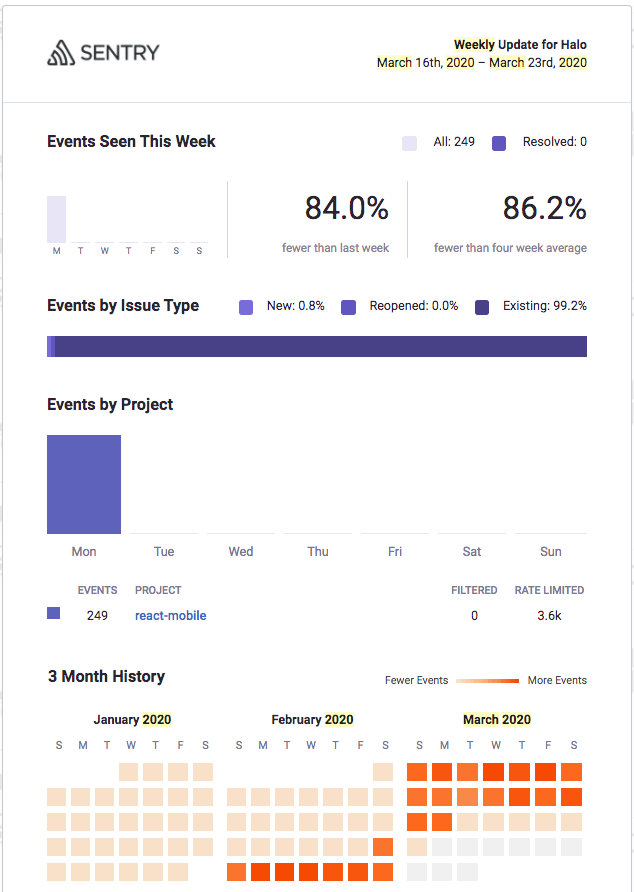
\includegraphics[width=\textwidth]{images/localhalo/sentry-weekly-report-16-mar-2020.png}
  \captionof*{figure}{\nth{16} -~\nth{22} March 2020}
  \label{fig:localhalo-sentry-weekly-report-16-mar-2020}
\end{minipage}\hfill%
\begin{minipage}{.45\textwidth}
  \centering
  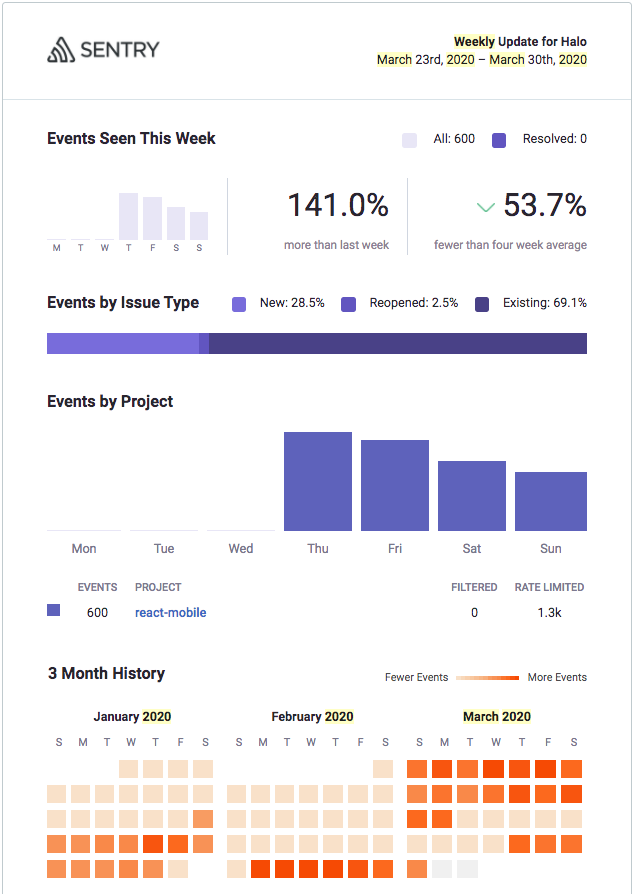
\includegraphics[width=\textwidth]{images/localhalo/sentry-weekly-report-23-mar-2020.png}
  \captionof*{figure}{\nth{23} -~\nth{29} March 2020}
  \label{fig:localhalo-sentry-weekly-report-23-mar-2020}
\end{minipage}
    \caption{Missing data reported in Sentry, in March 2020}
    \label{fig:sentry-missing-data-march-2020}
\end{figure}


\subsection{Developer experience}~\label{section-developer-experience-ux-design}
After the end of the cases studies, nonetheless of relevance, in June 2022 Google released Canary 3 of the integrated development environment (IDE) called Android Studio Electric Eel. This includes the facility to directly see and work with crashes reported by Firebase Crashlytics within the IDE. This makes the analytics information immediately and continuously available to the developers rather than relying on them visiting the Crashlytics website. It aims to reduce context switching and also encourage faster investigation and remediation of crashes~\citep{android2022_firebase_crash_integration_into_android_studio_electric_eel}.

\subsection{Meta-data}~\label{section-meta-data}
Meta-data may help developers with bug localisation and reproduction pertaining to the device model, its underlying hardware characteristics, the release of the platform, and so on. 

Figure \ref{fig:fabric-crashlytics-privacy-policy} provides an illustration of the privacy policy for Fabric Crashlytics which lists various the meta-data it collected at the time. The successor Firebase Crashlytics lists similar data being collected for crashes~\url{https://firebase.google.com/support/privacy#crash-stored-info}. The details of why these details were necessary was discussed online~\citep{kim2017_what_information_does_crashlytics_collect_from_end_users}.

\begin{figure}
    \centering
    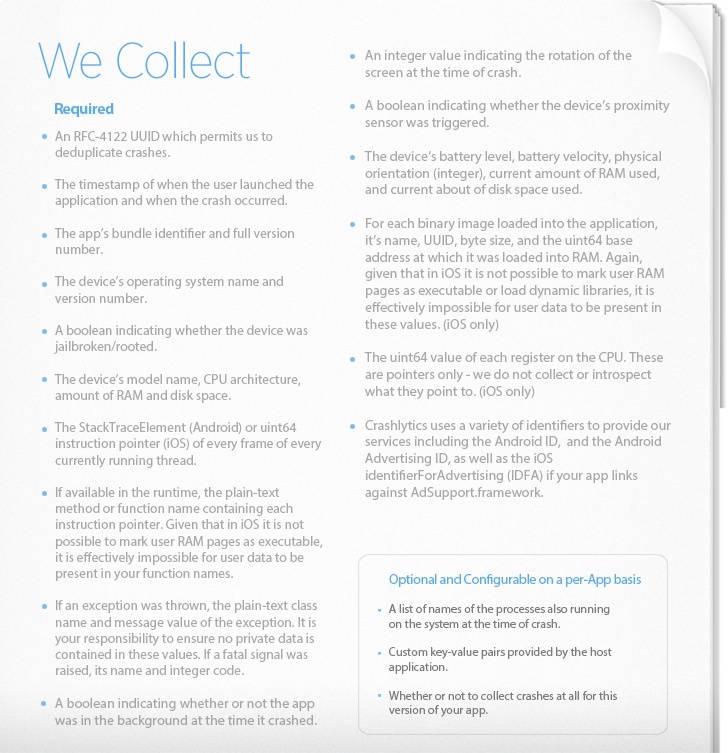
\includegraphics[width=10cm]{images/fabric-crashlytics/crashlytics-privacy-policy-38154ffbd69ef44a478b54365dc9b3ad.png}
    \caption{Fabric Crashlytics Privacy Policy (in 2015)\\{source: \tiny \url{https://web.archive.org/web/20150405071731/http://try.crashlytics.com/security/}}}
    \label{fig:fabric-crashlytics-privacy-policy}
\end{figure}

However, some app developers may receive data they didn't expect, particularly if they migrated from Fabric Crashlytics to Firebase Crashlytics. 

To provide some additional context Fabric and Firebase both offered facilities to combine various datasets into their reporting, for instance based on advertising SDKs. This led to reports that include demographics in addition to the crash analytics, \emph{etc.}~\footnote{Discussions on how the demographics are captured and made available include~\citep{joe2016_firebase_analytics_demographics} and~\citep{chelo2020_firebase_does_not_collect_age_or_gender_data}.}. 

The forced migration from Fabric Crashlytics to Firebase Crashlytics had two stages, the first was to migrate the project to the Firebase user interface and the second was to replace the Fabric SDK with the Firebase SDK. The Firebase SDK automatically collected additional data~\citep{firebase_help_GA4_2021_predefined_user_dimensions}.

As mentioned in the previous chapter, the Catrobat project chose to stop using Firebase Crashlytics when they discovered the demographics of the end users was also being recorded. 

In collaborative research into using Firebase Analytics for logging, 50 of 107 active Android opensource projects initialised just the Firebase Analytics SDK, they did not use any other aspect of the SDK~\citep{harty2021_logging_practices_with_mobile_analytics}~\footnote{Perhaps they thought that `Getting Started' was all they needed to do? or perhaps the default data was `good enough'?}. Therefore the contents and the limitations of the default meta-data are of particular interest since it is all those developers would have available to them. The remaining 57 projects used additional API calls to record additional information on one or more code-paths in the respective app.

\subsection{Engineering challenges}~\label{section-engineering-challenges}
Engineering challenges for mobile analytics include:
\begin{itemize}
    \item Support of collecting information from native code. This can be particularly pertinent for apps that include libraries in native code that are provided by third-parties.
    \item Collecting information from the earliest stage of app startup to the apps shutdown, otherwise data collection is incomplete.
    \item Establishing and maintaining sufficient information to calculate and provide sufficiently accurate comparisons, ratios, and so on. As an example, determining the Probability of Failure On Demand (\href{glossary-pfod}{PFOD}), requires counts of non-failures - those events/transactions/\emph{etc.} that \emph{worked}. Also, the sources/inputs/conditions that contributed to the failure may be useful to the app developer, does the mobile analytics SDK collect these? In the Kiwix case study, there were various sources of WebView crashes, these needed to be identified in order to attempt to prevent similar crashes in future.
    \item For the Vitals Scraper utility developed as part of this research, there were engineering challenges in first developing and then maintaining an automated interface to obtain reports and related information from Google Play Console and Android Vitals.
    \item For platform tools, collecting pertinent information across the process boundary includes engineering challenges. For in-app analytics, collecting information, such as ANRs, was a challenge during the period of the active app-centric case studies. 
\end{itemize}

\subsection{Vying for the attention of developers}~\label{section-vying-for-devs-attention}

Mobile Analytics tools compete for finite attention developers are able to provide. They vy for developers' attention to be selected and if selected then they vy for attention on an ongoing basis in order to communicate their alerts, reports, \emph{etc.} Pricing, licensing, and management approvals sometimes prevent some development team members from being able to use the tools directly.

\begin{itemize}
    \itemsep0em
    \item Access and use of mobile analytics tools allows them to be used interactively, where this is impractical copies, extracts, \emph{etc.} of reports and related material helps  preserve them for future analysis, for evidence, and so on. These copies and extracts can also extend the reach to people who don't have direct access to the tools. Several of the app-centric case studies, including Kiwix, Catrobat, LocalHalo, and the Commercial project limited access to various tools to a subset of the developers. In contrast, Moonpig, provided access to every member of the development team who had access to the source code of the app.
    \item When the analytics tools lack the attention of developers the effects of existing and new issues propagate and may enable these issues to snowball. The Kiwix project provided a good example of this with the loss of the lead developer for the Android app.
    \item The majority of the app-centric case studies used multiple mobile analytic tools. Some of the developers chose to ignore aspects of particular tools, for instance the crash analytics in Android Vitals in favour for similar services from other tools, even though Android Vitals is able to record some crashes that the other tools do not capture \emph{e.g.} owing to limitations in the respective SDK. The tools need to convince developers of the merits of their reports. The Moonpig development team, in particular, checked the reports of multiple tools to reduce their blind-spots.
    \item The LocalHalo project illustrated the flip-flop of failures between two analytics tools. This was insightful and demonstrates the value of having a combination of platform-level and in-app analytics, at least for apps written in frameworks such as react-native.
\end{itemize}


\section{Fit-for-purpose}~\label{section-fit-for-purpose}
Simply put, the mobile analytics tools need to be fit for purpose. They need to fit the needs/desires of the developers (product fit), provide actionable reports and a good return on any investment the developers make in terms of using the tools. When they integrate into the workflows of the developers they're more likely to be adopted as long term companions. Fidelity and ethical considerations bridge both fit-for-purpose and dependability.

{\small
\begin{itemize}
    \itemsep0em
    \item \sout{Product Fit: whether, and if practical how well, the mobile analytics product fits the desires/needs of the developers and their organisation.}
    \item \sout{Actionable Reports: reports the developers can action in order to address concerns presented in the reports.}
    \item \sout{Integration into workflows: the ability of a given mobile analytics tool/service to be integrated into development team's workflows.}
    \item Ethical considerations: the data collected by mobile analytics may have ethical implications a) for the operator/provider of the service, b) for their partners and customers, c) for the developers, d) for end-users. In this research our main focus is on the implications for the developers, nonetheless the other aspects are also important.
    \item Return On Investment (ROI): developers may make both implicit and explicit choices on what to invest in, for instance in terms of their focus, their effort, and their money. The analytics tools need to convince developers a) to invest and then b) whether to increase that investment (and if so what forms of investment e.g. in terms of writing more code, spending [more] money, using the tool more, etc.).
    \item Fidelity: an accurate, faithful representation.
\end{itemize}
}

\subsection{Product Fit}
\textbf{Product fit} addresses whether, and if practical how well, the mobile analytics product fits the desires/needs of the developers and their organisation. It is similar, but more specific than product/market fit~\footnote{\url{https://en.wikipedia.org/wiki/Product/market_fit}} - or conversely the market is pico-sized, gauged at the level of a development team. % See also concepts from https://en.wikipedia.org/wiki/Lean_startup e.g. actionable metrics.

Developers of mobile analytics tools, such as Iteratively~\footnote{Iteratively was acquired by Amplitude in 2021 and the products have been enhanced and integrated into Amplitude's product suite.}, seek ways to identify and determine what app developers will find useful. In Iteratively's case they used various techniques including `ten dots', illustrated in Figure \ref{fig:iteratively-product-market-fit}, during one-to-one semi-structured interviews to help Iteratively prioritise the features they developed and provided. Each interviewee was given the opportunity to complete this exercise, an example of their `dot-voting' is also provided in Figure \ref{fig:iteratively-product-market-fit}.\pending{Consider whether to include the analysis of the dot-votes (currently in the relevant empirical studies chapter).}

\begin{figure}[htbp!]
\centering
\begin{minipage}{.45\textwidth}
  \centering
  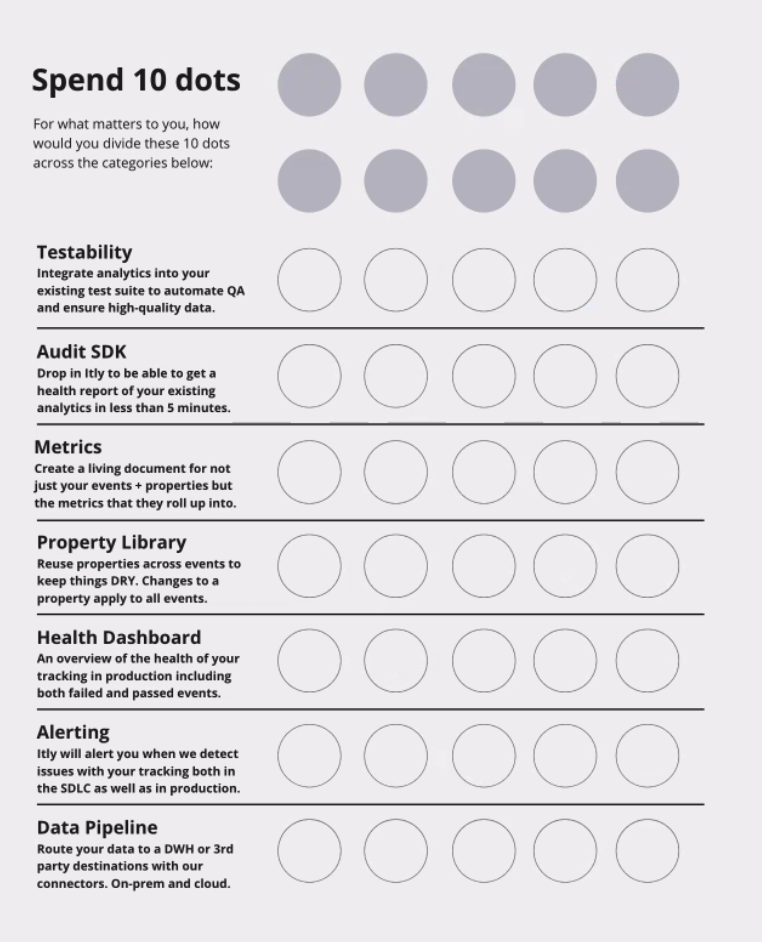
\includegraphics[width=\textwidth]{images/iteratively/spend-10-dots.png}
  \captionof*{figure}{Spend ten dots}
  \label{fig:iteratively-spend-ten-dots}
\end{minipage}\hfill%
\begin{minipage}{.45\textwidth}
  \centering
  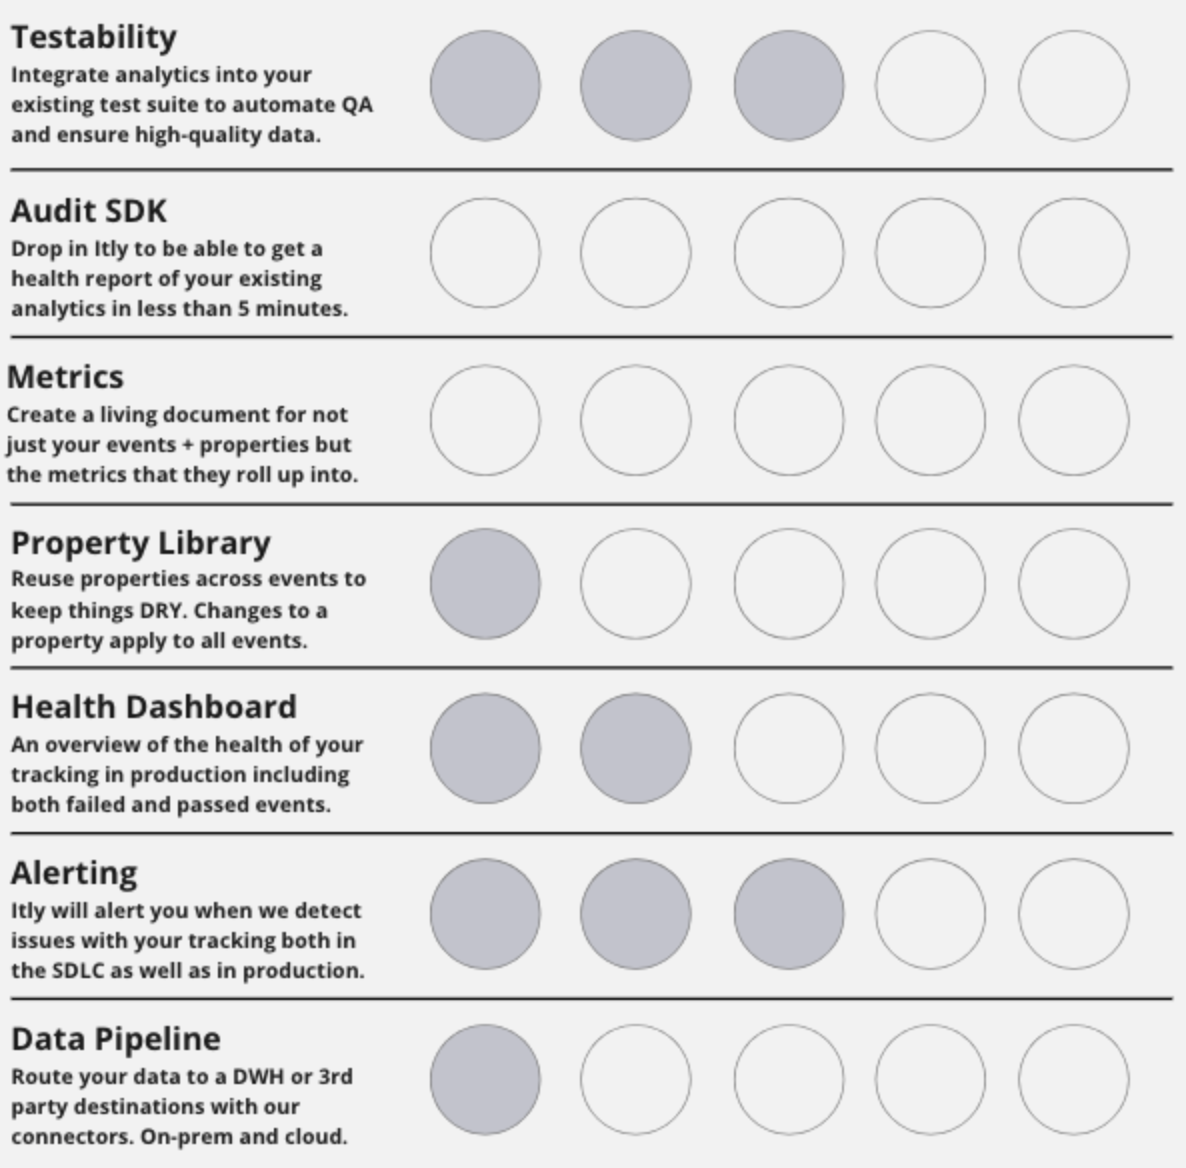
\includegraphics[width=\textwidth]{images/iteratively/dot-voting-example.png}
  \captionof*{figure}{Dot-voting example}
  \label{fig:iteratively-dot-voting-example}
\end{minipage}
    \caption{Iteratively: Product/Market fit}
    \label{fig:iteratively-product-market-fit}
\end{figure}

\textbf{Iteratively} had developed a combination of an online design tool that created a schema for third-party in-app analytics tools. They also provided build tools and a small client-side SDK (\textit{i.e.} a mobile SDK) which validated the schema had been implemented adequately in the mobile app. %, where all the data from the schema and only the data from the schema would be collected by the relevant mobile analytics SDK.
Iteratively's SDK was intended to limit the collection to only the data contained in the schema which was intended to stop the collection of other data (such as PII data). Through the use of the SDK, the build tools, and the online design tool development teams and their colleagues with other roles such as marketing, product, and so on could have a consistent and coherent understanding of the data that was being collected. Of interest to this research, they did not address the collection of errors or failures such as crashes in their SDK.

\textbf{LocalHalo} are a good example of a small development team who chose to include several mobile analytics SDKs into their mobile app where each SDK (and the respective service) was chosen to provide orthogonal data. They chose \href{https://sentry.io/}{Sentry} for technology facing analytics and \href{https://mixpanel.com/}{mixpanel} for product (business facing) analytics. Although Sentry provides APIs~\footnote{\url{https://docs.sentry.io/api/}} for integration and data forwarding~\footnote{\url{https://docs.sentry.io/product/data-management-settings/data-forwarding/}} and mixpanel provides data pipelines~\footnote{\url{https://mixpanel.com/data-integrations/}} LocalHalo did not use these. In contrast for the large commercial project data integration was deemed vital by the organisation in order to facilitate ongoing and \emph{ad-hoc} analysis across multiple sources of information. 

In the case of the \textbf{corporate project} the product (the mobile analytics tool) also had to fit at the level of the engineering organisation where the mobile analytics needed to be ingested into the corporation's `data-lake'. 

Finally for this topic, despite many mobile analytics SDKs, there may be situations where none provides the answers the developers seek. As a concrete example, \textbf{Smartnavi} uses Firebase and Google Analytics, mainly for tracking the popularity and the use of the app's features. The app also incorporated Fabric Crashlytics for crash reporting. Nonetheless the developer explained none of these analytics products provided analytics related to software running in the background, as a background process on Android. Smartnavi provides GPS services to other apps and runs in the background. As the Android Platform has evolved Google has embedded restrictions that limit and constrain background processes which meant the Smartnavi software is suspended (paused) by Android. The developer would like to improve the app's behaviours when it runs in the background but lacks the analytics to do so.


\subsection{Actionable Reports}
\textbf{Actionable Reports} are reports the developers can action in order to address concerns presented in the reports. % c.f. actionable metrics https://effectivesoftwaredesign.com/2021/03/23/lean-startup-principles-vanity-metrics-and-actionable-metrics/

Several of the app-centric case studies materialised because the respective development teams became aware of excessive and chronic error rates for their mobile apps. % Kiwix, Catrobat, C1
These projects had not managed to materially reduce the high crash rates directly and they were happy to receive help and insight in how to apply the information from the reports in their work. At the time they lacked the wherewithal to do so unaided, with interventions, including those that were part of this research, each of the development teams were able to materially improve the error rates of their respective apps.

None of the currently available mobile analytics tools seen during this research were able to pinpoint the causes of failures, instead they identify one or more effects \emph{e.g.} the app crashes, or is stopped by Android because it became unresponsive. The action-ability comes in part from the meta-data collected by the various mobile analytics tools which helped in bug localisation and in part from the characteristics and patterns contained in the reports. The Moonpig developers, for example, were sometimes able to identify a highly likely reason for the failure from the contents in the reports. They took action by modifying the application's source code.

Android Vitals aims to highlight emerging problems for instance if there is an acute and significant increase in the crash rate for the production release(s). It also provides cross-connections between problems found in Google Play's pre-launch reports and failures that occur in production. Developers found some of the reported failures easy to comprehend and address, others have been much less tractable. Several of the developers who use Crashlytics said they preferred using it over Android Vitals for comprehending crashes. Crashlytics provided more information than Android Vitals and the reports were easier to digest therefore the Crashlytics reports were more actionable than those from Android Vitals.

As discussed in the flaws topic (\secref{section-flaws-in-the-analytics}, \secref{section-flaws}) various reports have flaws, for instance in their aggregation. There is scope to improve the mobile analytics tools through improving the matching process in the data aggregation (for instance, where there are fragmented `failure clusters') and in the analysis across multiple legitimate failure clusters (such as across all \texttt{NullPointerExceptions}) to help identify underlying flaws in the development of the app.

\textbf{Moonpig} provides an illustrative example of how the development team was able to take proportionate and measured action as the crash-rate of their Android app increased. The cause was related to a known and documented issue with a third-party software library, RoboSpice. There was a clear correlation where the crash-rate increased on newer Android releases. The team was able to evaluate and estimate an appropriate timescale to replace that library by revising the application's source code. They were able to schedule the release to suit other strategic objectives rather than rushing to push out a `fix' of the app.

The release management reports in Google Play Console (that incorporate various Android Vitals reports pertinent to the latest release for the 7 days post release) were highly actionable for the Commercial project. The development team were able to abort releases that had unexpected increases in failure rates before those flawed releases adversely affected swathes of the userbase.

\subsection{Integration into workflows}~\label{section-integration-into-workflows}
Integration into workflows is the ability of a given mobile analytics tool/service to be integrated into development team's workflows. These workflows include bug tracking and release management. Some mobile analytics tools provide facilities where developers can mark and/or annotate elements in the reports, for instance to remove a crash cluster from the main report or to provide a bug-tracking link to help the developers streamline their work when using mobile analytics.

The\pending{Possibly move the following 3 paragraphs to the analytics in use chapter as I'm discussing what the teams did.} 
majority~\footnote{Moodspace and LocalHalo did not provide any details of their bug tracking processes.} of the app-centric case studies partly integrated mobile analytics reports into their bug tracking process by storing at least some of the contents of the reports some of the time.  
Of the projects that recorded the failures found by mobile analytics, it appears the Catrobat project use the crash's stack trace without anything else of the crash cluster's details or analytics~\footnote{Examples include: \href{https://jira.catrob.at/browse/CATROID-1025}{Issue CATROID-1025} and \href{https://jira.catrob.at/browse/CATROID-1030}{Issue CATROID-1030}.} Moonpig stated they recorded many of the failures however sometimes they short-circuited the bug tracking system and modified the source code directly where the likely fix was believed to be easy to address with minimal risk. As they monitored the various mobile analytics services assiduously post-release they had at least one safety-net, also they may have recorded pertinent information in their source code repository - as this was not available during the research it is impractical to check at this stage.

As Kiwix, Catrobat, LocalHalo, and perhaps other projects only provide a subset of the development team access to the mobile analytics services the rest of the team are blind to any reports or issues \textit{unless someone who has access provides the relevant information in the bug tracking system}. The GTAF project team record crashes reported by Firebase in their bug tracking system however they only embed the URL, they have not included copies of the pertinent details.

When cross-references are stored in mobile analytics viewers can see which of the issues have been reported (and by inference which have not been acknowledged e.g. because the issues are new to the team). The commercial project included terse notes in some, not all, of the crash clusters, sadly it was impractical to determine the criteria for the various behaviours by the developers. 

\begin{figure}
    \centering
    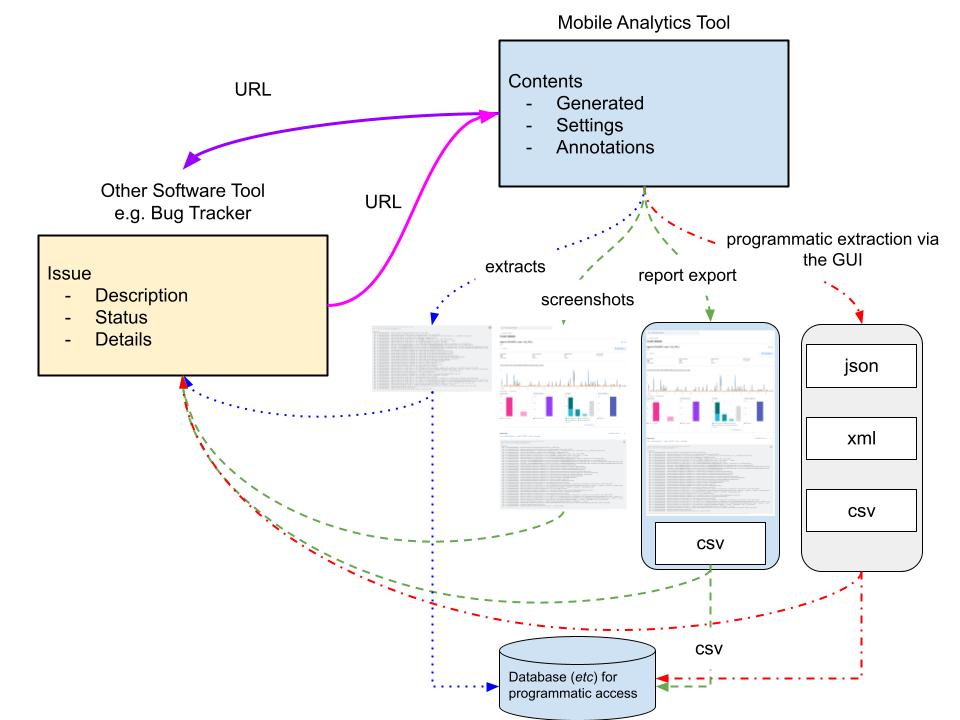
\includegraphics[width=\textwidth]{images/rough-sketches/integration-of-mobile-analytics-tool.jpeg}
    \caption{Addressing the contents of Mobile Analytics reports\\Source: Google Drawing \href{https://docs.google.com/drawings/d/1y7QP8UK7ugl0DzWIeH4udRxwsVMHjyQ6Am0qW6glkdE/edit?usp=sharing}{online here}.}
    \label{fig:addressing-the-contents-of-mobile-analytics}
\end{figure}

Figure \ref{fig:addressing-the-contents-of-mobile-analytics} illustrates various aspects of integration between mobile analytics and other software tools such as bug trackers. The mobile analytics tool provides reports in a graphical user interface. On the web the report has a URL (it may not be directly addressable in a mobile app equivalent tool) and visiting the URL with a suitably authenticated account results in the report being rendered if the mobile analytics service is working adequately. The mobile analytics tool \emph{may} provide interactive elements in the report page, for instance to hide the issue, to annotate the report, to modify the selection criteria. 

Some tool's URLs include structural elements for instance to vary the dates or the duration of the report (24 hours, 7 days, \emph{etc.}). And some tools provide for easy export of elements of the report or of the entire presentation of the report \emph{e.g.} as a PDF file or an image file. Another approach, albeit one seldom supported officially is to write code to extract content programmatically; we did so as part of this research and developed vitals-scraper to extract content from Android Vitals. 

\textbf{Why do these aspects matter?} 
Development teams often want to identify and track bugs including any code changes made with the aim of fixing the bug. Mobile analytics may be the source for the information about the bug and when the issue in the bug database includes pertinent information from the mobile analytics tool the development team can use that information to help understand the bug. The ability to cross-link the mobile analytics report and the issue in the bug tracker can enable team members to review the current, live information in the peer system. 

Figure \ref{fig:addressing-the-contents-of-mobile-analytics} includes five distinct mechanisms to integrate individual reports, or at least some of their contents.
\begin{enumerate}
    \itemsep0em
    \item The web address or URL: for some reports the URL may include structural elements that affect the contents of the report.
    \item Exports of the report: these are generally as a PDF or as a CSV file (which would include a subset of the entire report).
    \item Ubiquitous screenshots: some web browsers \emph{e.g.} Google Chrome limit the screenshot to the viewport (what's visible in the web browser), others \emph{e.g.} Firefox provide options to take a screenshot of the entire report.
    \item Content extracts: \emph{e.g.} using copy+paste links on screen, \emph{e.g.} Android Vitals does so for the stack trace of crashes and for the thread dump of ANRs.
    \item Programmatic extraction via the GUI: commonly known as screenscraping\footnote{Note: some mobile analytics tools may provide API access to obtain the reports and/or the contents of the reports however none was discovered during the case studies.}. 
\end{enumerate}

Text-based content can be stored and processed relatively easily (analysis and processing of Visually based PDF reports and images is beyond the scope of this research). Android Vitals provides various exports as files of comma-separated values (CSV files) however these are encoded in a UTF-16 character encoding, a seldom used encoding used by less than 0.005\% of websites according to~\citet{w3techs_utf16}, via~\citep{wikipedia_utf16}. UTF-16 content proved awkward to parse programmatically which complicates and adds friction to any analysis or integration of these CSV reports from Android Vitals.

The URLs may point to persistent historical reports or to recent, periodically updated, reports. Some reports are also updated as new releases of an app go into production. The URLs and/or the contents often have a finite life. Trend analysis might be available within the mobile analytics tool, otherwise it can be performed using snapshots of reports for a range/set of consistent periods \emph{e.g.} snapshots taken on the first day of every week can be used to perform trend analysis. Retention policies applied by the mobile analytics service may mean the underlying data is deleted; for example Firebase Crashlytics only retains crash stack traces, \emph{etc.} for 90 days~\citep{firebasesupport2022_crashlytics_data_retention_policy}. The data is then deleted from Firebase Crashlytics. Therefore, development teams would need to preserve the contents of the reports if they wish to perform longer-term analysis or for auditing, \emph{etc.}

Of all the mobile analytics tools covered in this research Iteratively uniquely focused on the design and verification that the mobile analytics captured the intended data. Their various software tools helped the teams design and implement the desired mobile analytics correctly in a mobile app. Their tools were primarily involved before the app was tested or released, nonetheless they included a short duration view of the mobile analytics events being emitted by the app when the app was being used.

In comparison, the release management section of Google Play Console is integrated into the rest of the services and reports offered in Google Play Console. Therefore it \emph{knows} the details of each release and is able to perform calculations and analysis accordingly for every new release of an app. In the commercial project the product owners were also able to use the release management reports to help them work with the developers to make decisions on staged rollouts including, when necessary, stopping the rollout entirely. The release management tools were a core part of release management and rollout for the overall team. % C1: Release management functionality including reports, alerts, history, and so on can enable developers to understand what's happening in terms of the adoption and use of their app releases. 

\textbf{iTools}: 
Two aspects of improving the integration of mobile analytics into development practices. These are:
\begin{itemize}
    \itemsep0em
    \item The ease of sharing pertinent information between the mobile analytics service, issue tracking, and to the developer's IDE~\footnote{And possibly integration with various collaboration tools such as Slack, Microsoft Teams, and so on would also be beneficial?}. %Persistent locators and data.  Cross-referencing in mobile analytics so viewers can see which of the issues have been reported (and by inference which have not been acknowledged e.g. because they're new to the team). Discuss improvements in these areas.
    \item How can mobile analytics reporting help developers to tackle and fix more of the failures? The GTAF case study provided an insightful example where the developers sometimes avoided addressing `difficult' failures. Perhaps, a service similar to GitHub's auto-suggestions integrated into mobile analytics and the developer's IDE could help reduce risk of exacerbating a situation by taking action (inaction is sometimes perceived as a safer course of behaviour than trying to tackle an issue and being seen to fail to do so).  
\end{itemize}

\subsection{Ethical considerations}
The data collected by mobile analytics may have ethical implications a) for the operator/provider of the service, b) for their partners and customers, c) for the developers, d) for end-users. In this research our main focus is on the implications for the developers, nonetheless the other aspects are also important.

\subsection{ROI}

\subsection{Fidelity}

\section{Utility}~\label{section-utility}

\begin{itemize}
    \itemsep0em
    \item Efficacy of the tool: how efficient and how effective is the tool, i.e. how efficacious is the tool? Did it achieve the objectives it claims to achieve?
    \item Benefits of combining tools: an observation of benefits developers can obtain through combining their use of several mobile analytics tools.
\end{itemize}



\section{Dependability}~\label{section-dependability}

\begin{itemize}
    \itemsep0em
    \item Flaws: weaknesses, mistakes, errors, etc. pertaining to the mobile analytics tool/service.
    \item Link rot, preservation of results: the validity of a URL may be finite, as may the contents be even if the link remains. For mobile analytics services link rot is often a common reason why results are no longer available from the mobile analytics service - the link was ephemeral. In such cases the results would need to be preserved while the results are still available. In some cases the rot may be easy to predict, for instance as data ages beyond the predefined date range of a report, in other cases less so, for instance when the active release is updated the data for the previous currently active release might 'disappear' from some reports.
    \item Testability: the ability to test the overall service, the tool, and/or components that comprise the analytics tool. 
    \item Trustworthiness: a measurement/assessment of the trustworthiness of the mobile analytics tool/service.
\end{itemize}

\subsection{Flaws}~\label{section-flaws}



\section{Some limits of what can be measured}

Here's a placeholder list, the points will need integrating.
\begin{itemize}
    \item React Native runtime - within runtime crashes vs. application crashes. (LocalHalo and Taskinator apps).
    \item Crashes at startup c.f. private correspondence with Google.
\end{itemize}

\section{Pre-launch reports}
The GTAF project uses pre-launch reports (an intrinsic part of Google Play Console), and the pre-launch report includes automated testing of pre-release apps. The crashes reported in pre-launch reports do not necessarily affect end users. Conversely the pre-launch report automated testing does not find all the failures that affect end users. (Dua \& Zikr app).

Why some projects stopped using pre-launch reports: c.f. the Google bug. TODO add link to the issue on Google and add supporting text.

\section{Flaws in the mobile analytics tools and/or services}

Since 2011, Google has published a list of various changes and corrections to Google Play Console~\citep{google_play_troubleshoot_app_statistics_problems}. During this research numerous additional were discovered that were not published by Google even though their engineering team acknowledged many of these flaws (they chose not to respond to the rest of the flaws). 

\section{Integration and the useful half-life of mobile analytics outputs}
Web-scraping of content from web-sites continues to be a frequent activity performed by many people and services. Web-scraping is used in many fields including bioinfomatics, where the authors discussed why web-scraping was still necessary in a world full of API's~\citet{glez2014_web_scraping_in_an_API_world}. A more recent paper by~\citet{diouf2019_web_scraping_state_of_the_art_and_areas_of_application} briefly presents various inefficiencies in web scraping. Curiously this paper singles out journalism as an under-served area despite it being written about 7 years earlier in Chapter 4 of~\citet{gray2012_the_data_journalism_handbook} (and also covered in a more recent version of the book,~\citet[on pages 133, 238]{bounegru2021_the_data_journalism_handbook}. Suffice to say, web-scraping is a topic that has been written about, albeit not in the context of scraping content from mobile analytics web interfaces. 

API access to mobile analytics has been requested previously~\citep{stackoverflow2013_getting_statistics_from_google_play_developer_console_with_an_api} and various people have developed code that interfaces with Google Play Console in an attempt to provide automated, scripted access to the content.

Our work in developing Vitals Scraper as an opensource project~\citep{vitals_scraper_github_package} and releasing it as an NPM package~\citep{vitals_scraper_npm_package} demonstrates the necessity, viability, and some of the maintenance challenges of writing automated software for web-scraping of outputs from Google Play Console with Android Vitals~\footnote{Note: there was another similar sounding opensource project \url{https://github.com/tmurakam/googleplay_dev_scraper} that provided mechanisms to automate the downloading of the \texttt{csv} monthly reports rather than the live reports. It was last updated in 2013 so no longer current.}. There was also the Andlytics opensource app that provided developers with access to data from their Google Play Console account~\footnote{\url{https://github.com/AndlyticsProject/andlytics}}, however this project also ceased active development for various reasons, probably because Google chose to restrict access to the underlying data in 2019~\footnote{\url{https://github.com/AndlyticsProject/andlytics/issues/766}}. % See also the historic posts by the project on Facebook for screenshots and updates https://www.facebook.com/Andlytics/


None of the mobile analytics tools encountered during the research provided complete access to the outputs using APIs. Furthermore, the ability to record and preserve copies of visual reports (as well as the underlying data) facilitates both practical use of the data in the field (for instance to record the information in an issues tracking database) and for further analysis and research. 

Enterprise-grade mobile analytics services provide mechanisms to export data to homogeneous data storage platforms~\citep{androiddevelopers2015_integrate_play_data_into_your_workflow_with_data_exports}; for instance Google Analytics tools export content to Google Cloud Storage~\footnote{\url{https://support.google.com/googleplay/android-developer/answer/6135870?hl=en-GB}}, and to automate the process~\footnote{\url{https://cloud.google.com/bigquery-transfer/docs/play-transfer}}. Microsoft App Center is unusually complete and provides a comprehensive set of open APIs \url{https://openapi.appcenter.ms/} as well as the ability to export analytics data to Azure \url{https://docs.microsoft.com/en-us/appcenter/analytics/export} and even export data for individual users \url{https://docs.microsoft.com/en-us/appcenter/gdpr/analytics-export}. Google Analytics provides various reporting APIs including those for Exceptions~\footnote{\url{https://ga-dev-tools.web.app/dimensions-metrics-explorer/exceptions}} which are collected by Firebase Analytics for both Android and iOS apps~\footnote{\url{https://developers.google.com/analytics/devguides/collection/firebase/android}}. % See also their github site that underpins the docs https://github.com/googleanalytics/ga-dev-tools

Some of the mobile analytics providers offer developers customisation options such as custom dashboards and reports in Sentry \url{https://docs.sentry.io/product/discover-queries/uncover-trends/}

As a broader observation, various companies provide app analytics services where they obtain the underlying data % See the discussion for https://stackoverflow.com/a/49893656/340175
and aim to provide easy to use, attractive, and actionable reports; examples include \url{https://appfigures.com/} and \url{https://www.data.ai/en/} (previously known as AppAnnie). Appfigures also publishes status reports for the performance of Google Play and Apple's App Store Connect service, these track the publishing performance of these two app stores; at the end of February 2022 they observed Google has been several days late publishing their free daily reports. % Screenshots have been recorded for posterity and are available in my research's appfigures.com folder. 

\section{Differences between mobile analytics tools}
Pocket Code incorporated in-app mobile analytics that recorded both crashes and errors (generally these errors are exceptions that \textit{are} caught and handled by the app) the case study provided the opportunity to study Fabric Crashlytics and to enable its outputs to be compared and contrasted with those from Google Play Console with Android Vitals. \textbf{TODO} discuss the differences.


\section{Improvements to Google Play Console with Android Vitals}

Direct quotes from the CTO of Moodspace (June 2019): \emph{``As for several things I think are missing:''}
\begin{itemize}
    \item \textit{``A gradle plugin to integrate play store uploading into CI processes. I currently use a 3rd party plugin to do this, but it would feel a little more secure if it came from Google.''}
    \item \textit{``Top line core vitals figures even if you don't have enough users!''}
    \item \textit{``Someway for testers to download old apks from either internal app sharing, or the internal release track.''}
\end{itemize}

And \emph{``Crashlytics only covers the crash report of Android vitals, so unfortunately there's no way to get things like battery usage of ANR reports unless Google makes those reports available :(. In terms of crashes, I'd always prefer Crashlytics to Android vitals, simply because there are added features like non-fatal reporting and logs which can make surfacing the cause of errors much easier (but do take need added effort to integrate compared to android vitals).''}

\section{Improving the integration and the useful half-life of mobile analytics outputs}
To discuss, APIs rather than Web Scraping, Persistent and timestamped links to reports (c.f. how github and wikipedia provide versioned links).

In late 2020 Google made various changes to Google Play Console, they provided the ability for developers to directly download individual stacktraces for crashes~\citep{stackoverflow2018_how_can_i_get_app_crash_log_from_google_play_console} which is a useful, small improvement (see \url{https://stackoverflow.com/a/49893656/340175}).


Sentry provides various tools to help development teams focus on key issues,  \url{https://blog.sentry.io/2021/04/20/silencing-distractions-with-review-list-and-automations} (I don't know what information is populated by Sentry when it creates JIRA tickets),  and on the health of new app releases: \url{https://docs.sentry.io/platforms/android/configuration/releases/#release-health}


\section{Discussion on mobile analytics tools and their artefacts}
Mobile Analytics tools need to evolve to remain current and to attract and retain users. Platform tools have a unique advantage compared to in-app tools as the platform tools can collect data across the entire population~\footnote{Subject to opt-outs, sampling, network connectivity, and other reasons the data wouldn't be sent from the overall population.}. For the Android platform, Google Play Console and Android Vitals are able to provide comparisons with apps of peers, both peers selected by app store classifications~\citep{androiddevelopersblog2021_gpc_powers_better_strategic_decisions_etc} and a custom set selected by the developer~\citep{play_console_help_compare_your_apps_android_vitals_and_ratings_with_peer_groups}. 

\section{Summary of tools and their artefacts}
TBC